% !TEX encoding = UTF-8 Unicode
\documentclass{beamer}
\usetheme{Szeged}

\usepackage{color}
\usepackage{url}
\usepackage[utf8]{inputenc}
\usepackage{graphicx}

\usepackage[english, serbian]{babel}

%\usepackage[unicode]{hyperref}
\usepackage{amsmath}
\usepackage{amsthm}
\usepackage{amssymb}
\hypersetup{colorlinks,citecolor=green,filecolor=green,linkcolor=blue,urlcolor=blue}
\usepackage[title]{appendix}
\usepackage{float}
\usepackage[graphicx]{realboxes}
\usepackage{chngcntr}
\counterwithin{figure}{section}
\usepackage{listings}
\usepackage{textcomp}
\usepackage{xcolor}
\usepackage{adjustbox}
\lstset {
    language=Java,
    frame=none,
    %xleftmargin=-.25in,
    %xrightmargin=.25in
    framesep=10pt,
    tabsize=4,
    showstringspaces=false,
    upquote=true,
    commentstyle=\color{gray},
    keywordstyle=\color{orange},
    stringstyle=\color{red},
    basicstyle=\scriptsize\ttfamily,
    emph={int,char,double,float,unsigned,void,bool},
    emphstyle={\color{blue}},
    escapechar=\&,
    classoffset=1,
    morekeywords={>,<,.,;,,,-,!,=,~},
    keywordstyle=\color{weborange},
    classoffset=0,
    breaklines=true
}

\usepackage[font=scriptsize,labelfont=bf]{caption}


\title{Kori\v{s}\'c{}enje Furijeovih redova za crtanje pomo\'c{}u epiciklusa}

\author{\href{mailto:ivan_ristovic@math.rs}{Ivan Ristović}}
\date{septembar 2019.}


\begin{document}
\begin{frame}
    \titlepage
\end{frame}

\begin{frame}{\v{S}ta su epiciklusi?}
    \begin{itemize}
        \item \emph{Epiciklus}, u prevodu sa gr\v{c}kog, zna\v{c}i \emph{na krugu}, tj. \emph{krug na krugu}
        \item Ptolomejev model kretanja nebeskih tela
    \end{itemize}
    \centering
    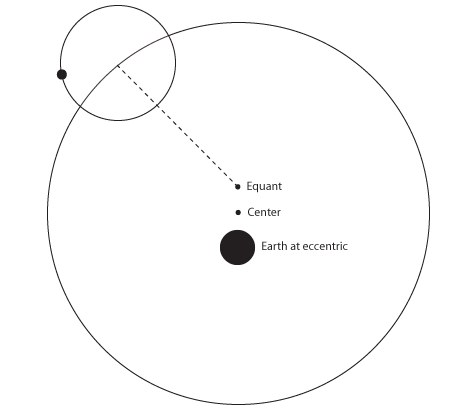
\includegraphics[scale=0.5]{images/ptolomaic_model.PNG}
\end{frame}

\begin{frame}{Kakve sve orbite mo\v{z}emo pratiti pomo\'c{}u epiciklusa?}
    \centering
    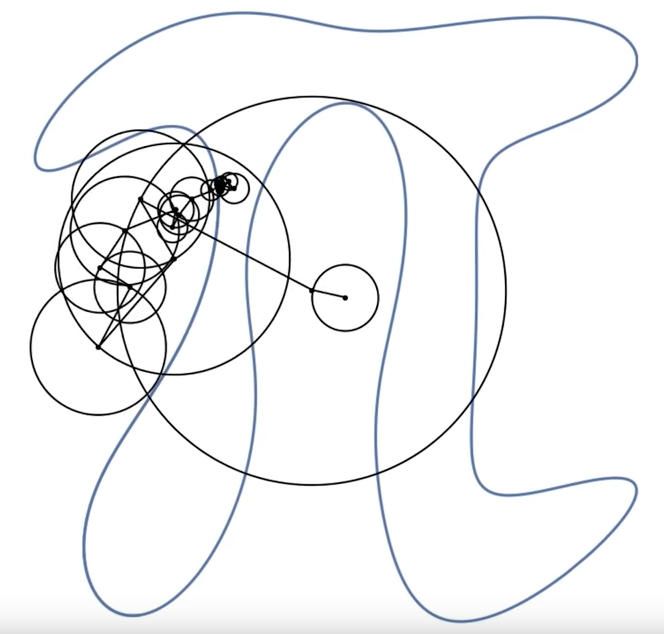
\includegraphics[scale=0.35]{images/ep2.PNG}
\end{frame}

\begin{frame}{Kakve sve orbite mo\v{z}emo pratiti pomo\'c{}u epiciklusa?}
    \centering
    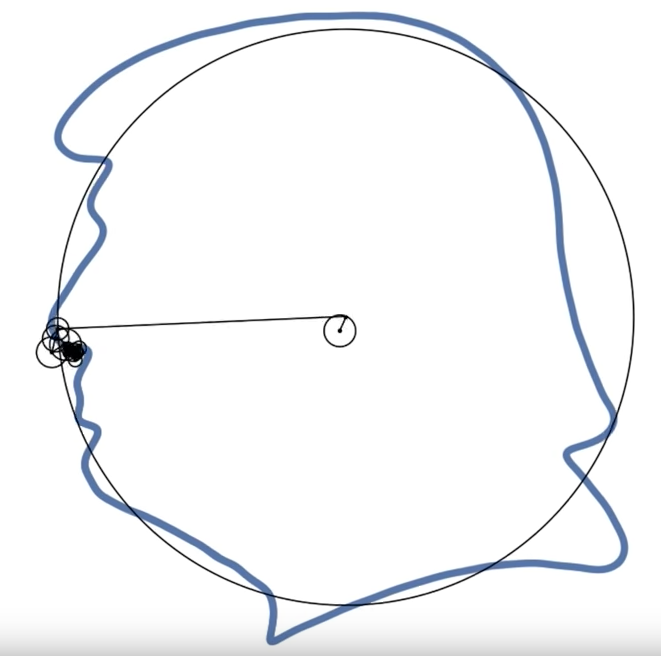
\includegraphics[scale=0.35]{images/ep1.PNG}
\end{frame}

\begin{frame}{Kako matemati\v{c}ki predstaviti epicikluse?}
    \centering
    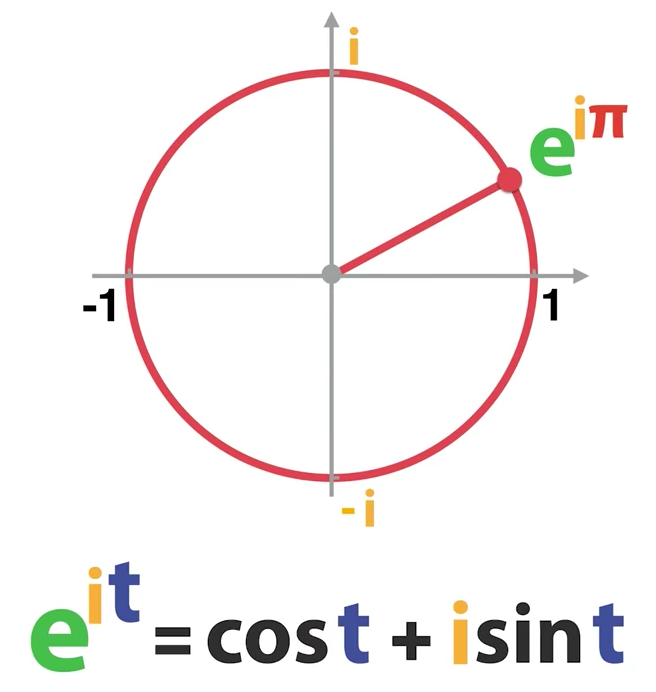
\includegraphics[scale=0.35]{images/ep3.PNG}
\end{frame}

\begin{frame}{Kako matemati\v{c}ki predstaviti epicikluse?}
    \begin{tabular}{cc}
        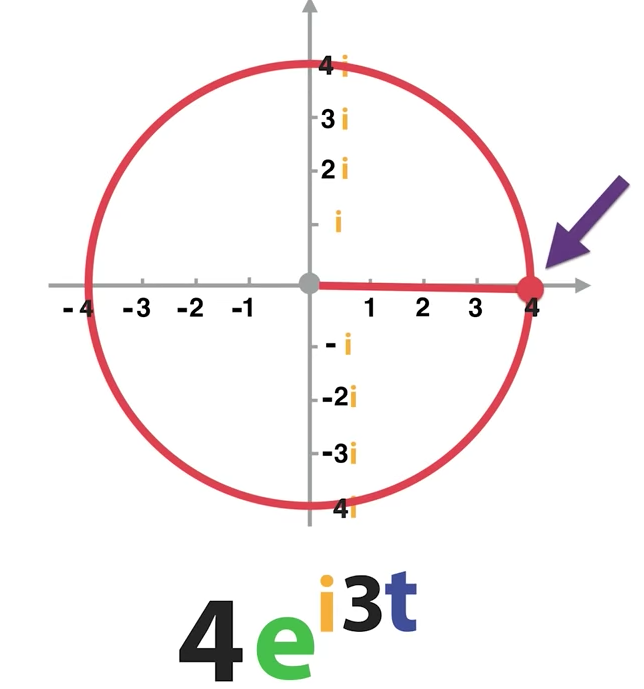
\includegraphics[scale=0.3]{images/ep4.PNG} &
        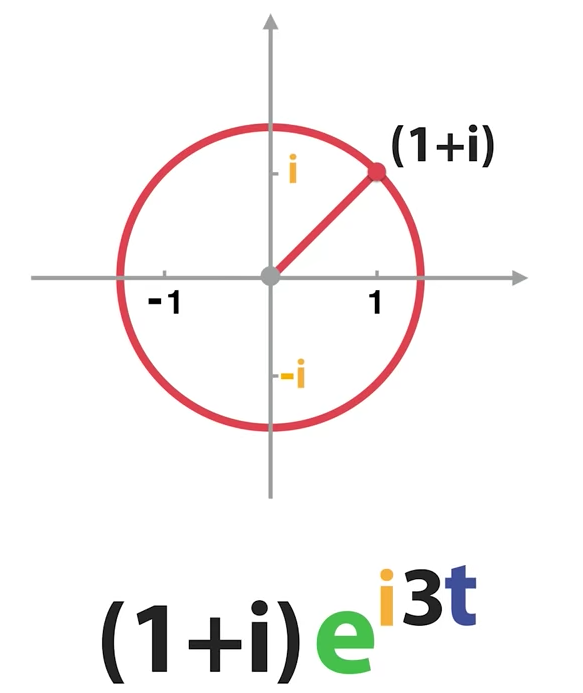
\includegraphics[scale=0.35]{images/ep5.PNG}            
    \end{tabular}
\end{frame}

\begin{frame}{Kako matemati\v{c}ki predstaviti epicikluse?}
    \centering
    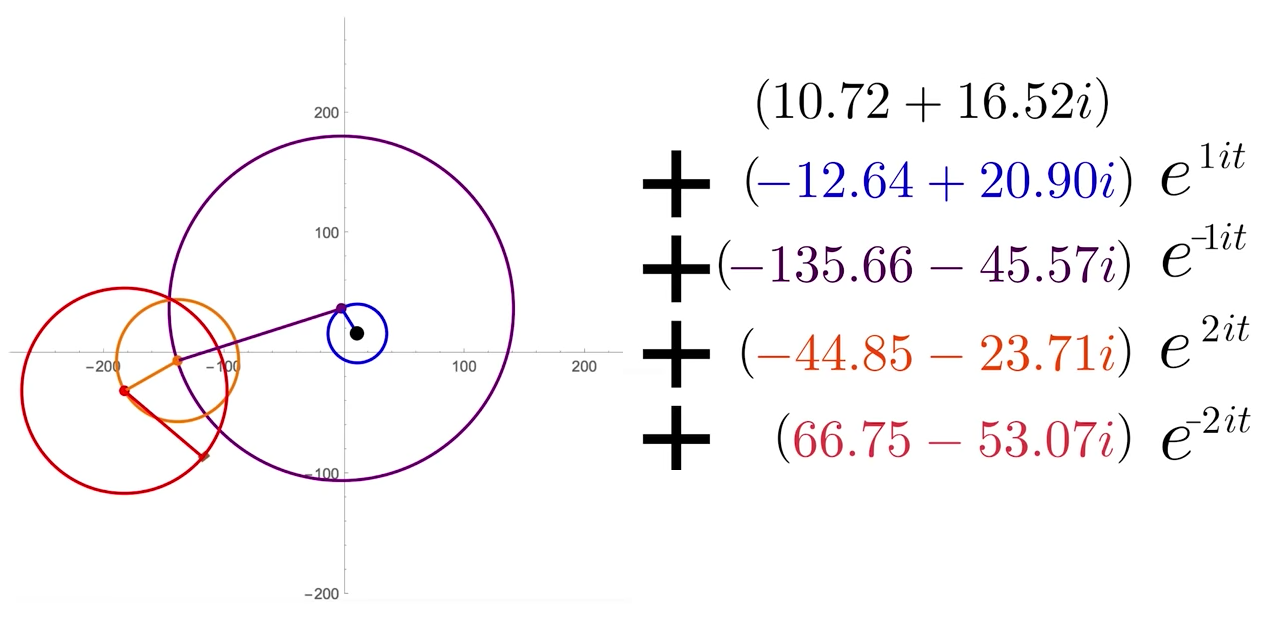
\includegraphics[scale=0.35]{images/ep7.PNG}
\end{frame}

\begin{frame}{Primetimo da...}
    \centering
    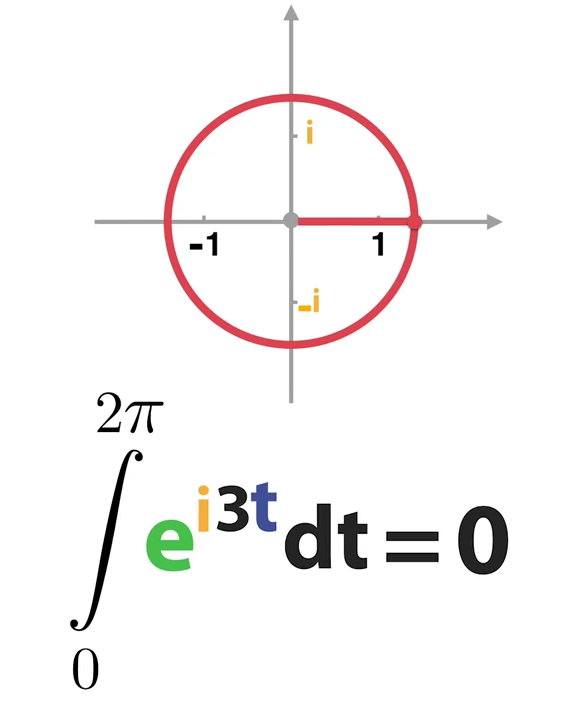
\includegraphics[scale=0.35]{images/ep6.PNG}
\end{frame}

\begin{frame}{Dakle, signal mo\v{z}emo predstaviti kao}
    \centering
    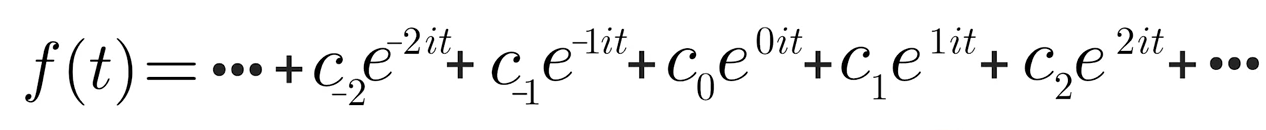
\includegraphics[scale=0.3]{images/ep8.PNG}
\end{frame}

\begin{frame}{Kako izra\v{c}unati $c_i$?}
    \centering
    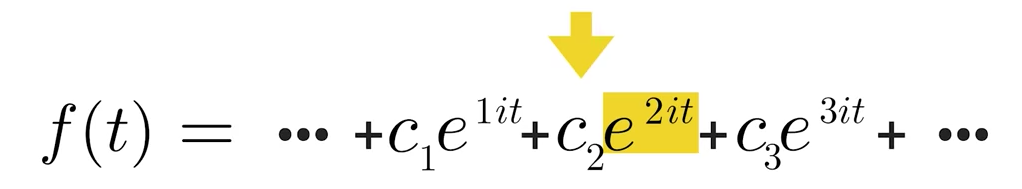
\includegraphics[scale=0.3]{images/ep9.PNG}
    %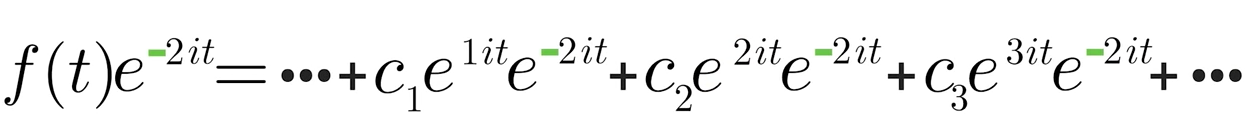
\includegraphics[scale=0.3]{images/ep10.PNG}
    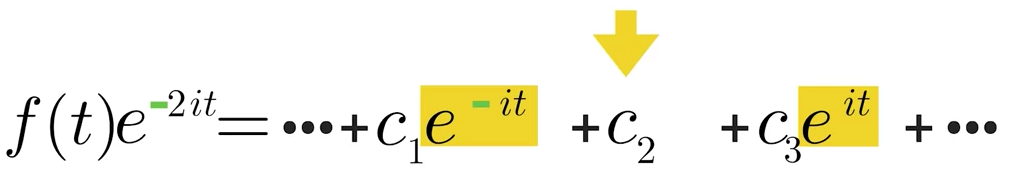
\includegraphics[scale=0.3]{images/ep11.PNG}
    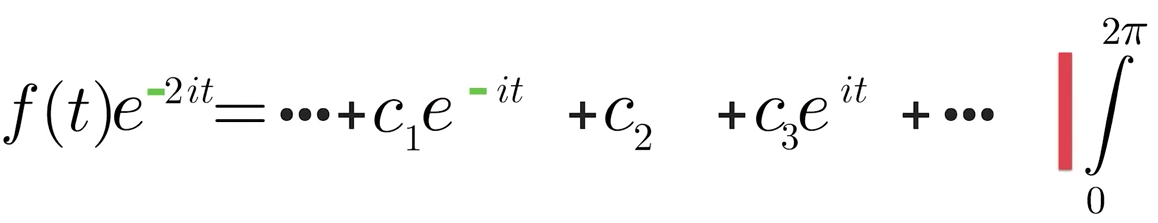
\includegraphics[scale=0.3]{images/ep12.PNG}
    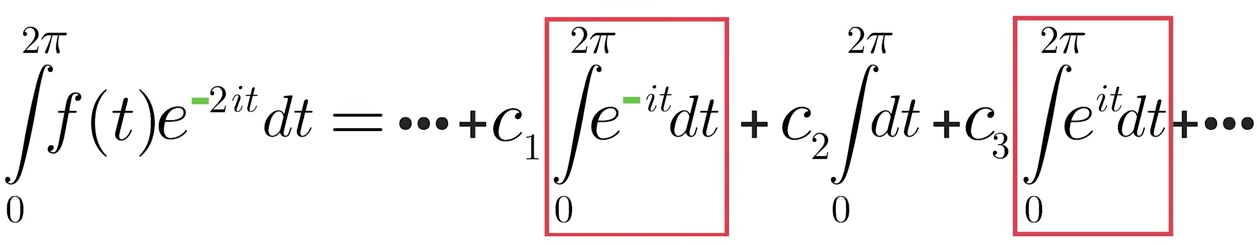
\includegraphics[scale=0.3]{images/ep13.PNG}
\end{frame}

\begin{frame}{Kako izra\v{c}unati $c_i$?}
    \centering
    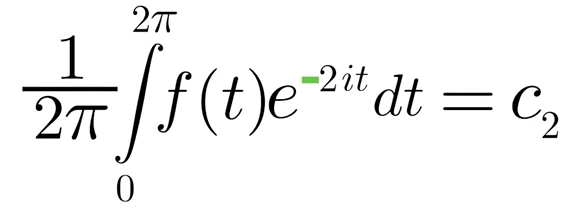
\includegraphics[scale=0.3]{images/ep14.PNG}
    \begin{itemize}
        \item Izgleda poznato?
    \end{itemize}
    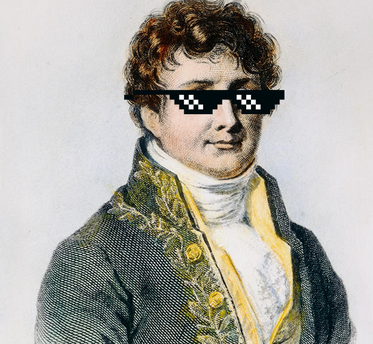
\includegraphics[scale=0.3]{images/fourier.PNG}
\end{frame}

\begin{frame}{Dakle...}
    \begin{itemize}
        \item Signal dobijamo u diskretnom obliku
        \item Iskoristimo DFT
        \item Dobijene kompleksne brojeve tretiramo kao epicikluse
        \item Iscrtamo 
    \end{itemize}
\end{frame}

\begin{frame}{Demonstracija...}
    \centering
    Demonstracija :)
\end{frame}

\begin{frame}{Pitanja}
    \centering
    ???
\end{frame}

\begin{frame}{}
    \centering
    Hvala na pa\v{z}nji!
\end{frame}

\begin{frame}{Materijal za slajdove pozajmljen od}
    \centering
    \url{https://www.youtube.com/watch?v=qS4H6PEcCCA}
\end{frame}


\end{document}